% Diagrama 2 — Abastecimiento y prorrateo (v2)
% =====================================================================
%  estilo.tex — sistema visual común de los diagramas RedPepper
%  Se incluye desde cada figura (documento independiente).
% =====================================================================
\documentclass[11pt,tikz,border=6pt]{standalone}

\usepackage[utf8]{inputenc}
\usepackage[T1]{fontenc}
\usepackage{lmodern}
\usepackage{helvet}
\renewcommand{\familydefault}{\sfdefault}

\usepackage{tikz}
\usetikzlibrary{positioning,arrows.meta,shapes.geometric,fit,backgrounds,calc}

% --- Paleta por rol (tonos suaves, legibles en impresión) ---------------
\definecolor{cCliente}{HTML}{FFF1D6}
\definecolor{bCliente}{HTML}{B8860B}
\definecolor{cCaja}{HTML}{E4F2E1}
\definecolor{bCaja}{HTML}{3E7D3A}
\definecolor{cSistema}{HTML}{E3ECF9}
\definecolor{bSistema}{HTML}{2F5D9E}
\definecolor{cCocina}{HTML}{FBE5E3}
\definecolor{bCocina}{HTML}{A33B33}
\definecolor{cAdmin}{HTML}{EDEDED}
\definecolor{bAdmin}{HTML}{555555}
\definecolor{cProveedor}{HTML}{F0E7F7}
\definecolor{bProveedor}{HTML}{6A4C93}
\definecolor{cContador}{HTML}{DEF1EF}
\definecolor{bContador}{HTML}{2E7D74}

% --- Estilos ------------------------------------------------------------
\tikzset{
  proc/.style={
    draw=black!55, rounded corners=3pt, fill=white, align=center,
    font=\small,
    execute at begin node={\hyphenpenalty=10000\exhyphenpenalty=10000},
    inner sep=3.5pt, minimum height=0.95cm, text width=3.05cm
  },
  cliente/.style={proc, fill=cCliente, draw=bCliente},
  caja/.style={proc, fill=cCaja, draw=bCaja},
  sistema/.style={proc, fill=cSistema, draw=bSistema},
  cocina/.style={proc, fill=cCocina, draw=bCocina},
  admin/.style={proc, fill=cAdmin, draw=bAdmin},
  proveedor/.style={proc, fill=cProveedor, draw=bProveedor},
  contador/.style={proc, fill=cContador, draw=bContador},
  dec/.style={
    diamond, aspect=2.1, draw=black!60, fill=white, align=center,
    font=\footnotesize, inner sep=1pt, minimum width=2.6cm, minimum height=1.15cm
  },
  ini/.style={
    draw=black!60, rounded corners=14pt, fill=black!6, align=center,
    font=\footnotesize\bfseries, inner sep=5pt, minimum height=0.9cm, text width=2.6cm
  },
  flecha/.style={-{Stealth[length=2.2mm,width=1.6mm]}, draw=black!70, line width=0.7pt},
  flechad/.style={flecha, dashed},
  etiqueta/.style={font=\scriptsize, inner sep=2pt, fill=white, draw=none, text=black!75},
  banda/.style={fill=black!82, text=white, font=\small\bfseries, align=center, inner sep=4pt},
  leyenda/.style={font=\scriptsize, align=left, text=black!80}
}

% --- Encabezado y leyenda ----------------------------------------------
% #1 ancho total, #2 título, #3 y del encabezado
\newcommand{\encabezado}[3]{%
  \node[banda, minimum width=#1, minimum height=0.62cm, anchor=north west]
    at (-0.45,#3) {\strut #2};%
}
% #1 x, #2 y  (leyenda en dos filas para evitar solapamientos)
\newcommand{\leyendaRoles}[2]{%
  \begin{scope}[shift={(#1,#2)}]
    \foreach \x/\c/\b/\t in {0/cCliente/bCliente/Cliente,
                              2.7/cCaja/bCaja/Caja,
                              5.2/cSistema/bSistema/Sistema,
                              8.4/cCocina/bCocina/Cocina}{%
      \node[draw=\b, fill=\c, minimum width=0.34cm, minimum height=0.24cm,
            anchor=west] at (\x,0) {};
      \node[leyenda, anchor=west] at ({\x+0.24},0) {\t};%
    }
    \foreach \x/\c/\b/\t in {0/cAdmin/bAdmin/Administración,
                              3.4/cProveedor/bProveedor/Proveedor,
                              6.6/cContador/bContador/Contador}{%
      \node[draw=\b, fill=\c, minimum width=0.34cm, minimum height=0.24cm,
            anchor=west] at (\x,-0.42) {};
      \node[leyenda, anchor=west] at ({\x+0.24},-0.42) {\t};%
    }
  \end{scope}
}


\begin{document}
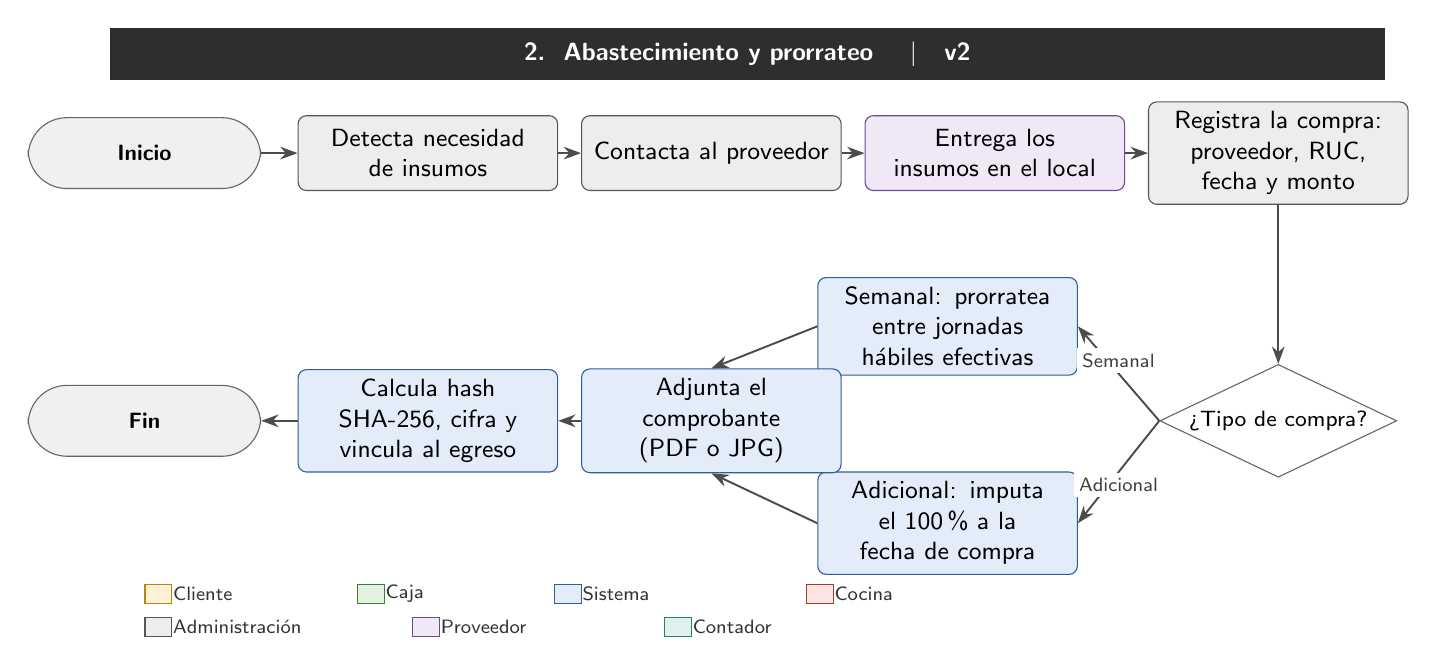
\begin{tikzpicture}

  \encabezado{16.2cm}{2.\ \ Abastecimiento y prorrateo \quad\textbar\quad v2}{1.6}

  % ---------------- Fila 1 ----------------
  \node[ini]       (ini) at (0,0)    {Inicio};
  \node[admin]     (p2)  at (3.6,0)  {Detecta necesidad de insumos};
  \node[admin]     (p3)  at (7.2,0)  {Contacta al proveedor};
  \node[proveedor] (p4)  at (10.8,0) {Entrega los insumos en el local};
  \node[admin]     (p5)  at (14.4,0) {Registra la compra: proveedor, RUC, fecha y monto};

  % ---------------- Decisión y ramas ----------------
  \node[dec] (d) at (14.4,-3.4) {¿Tipo de compra?};

  \node[sistema] (sem) at (10.2,-2.2) {Semanal: prorratea entre jornadas hábiles efectivas};
  \node[sistema] (adi) at (10.2,-4.7) {Adicional: imputa el 100\,\% a la fecha de compra};

  % ---------------- Fila 2 ----------------
  \node[sistema] (adj)  at (7.2,-3.4) {Adjunta el comprobante (PDF o JPG)};
  \node[sistema] (hash) at (3.6,-3.4) {Calcula hash SHA-256, cifra y vincula al egreso};
  \node[ini]     (fin)  at (0,-3.4)   {Fin};

  % ---------------- Flujo ----------------
  \draw[flecha] (ini) -- (p2);
  \draw[flecha] (p2)  -- (p3);
  \draw[flecha] (p3)  -- (p4);
  \draw[flecha] (p4)  -- (p5);
  \draw[flecha] (p5)  -- (d);

  \draw[flecha] (d.west) -- node[etiqueta, above, pos=0.5] {Semanal} (sem.east);
  \draw[flecha] (d.west) -- node[etiqueta, below, pos=0.5] {Adicional} (adi.east);

  \draw[flecha] (sem.west) -- (adj.north);
  \draw[flecha] (adi.west) -- (adj.south);

  \draw[flecha] (adj)  -- (hash);
  \draw[flecha] (hash) -- (fin);

  \leyendaRoles{0}{-5.6}

\end{tikzpicture}
\end{document}
